\documentclass[../improvements.tex]{subfiles}

\begin{document}

  論理合成の結果から, クリティカルパスが EX ステージにあることが分かった.
  そのクリティカルパスは図\ref{fig:critical-path-before}で示す.

  \begin{figure*}[h]
    \centering
    \begin{subfigure}{\columnwidth}
      \centering
      \resizebox{0.5\columnwidth}{!}{
        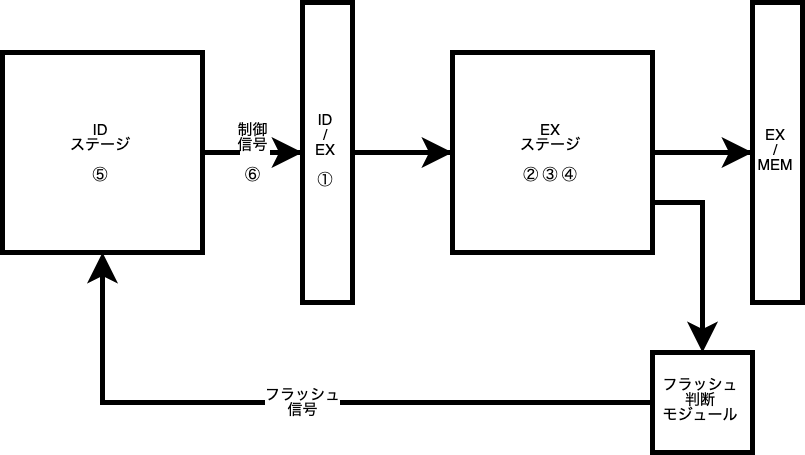
\includegraphics{../../images/critical_path_before.png}
      }
      \caption{改善前}
      \label{fig:critical-path-before}
    \end{subfigure}
    \begin{subfigure}{\columnwidth}
      \centering
      \resizebox{0.5\columnwidth}{!}{
        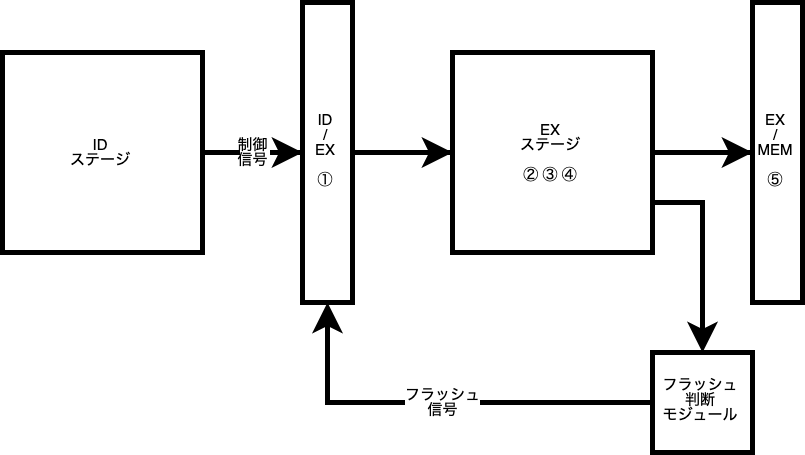
\includegraphics{../../images/critical_path_after.png}
      }
      \caption{改善後}
      \label{fig:critical-path-after}
    \end{subfigure}
    \caption{改善前後のクリティカルパス}
  \end{figure*}

  上記のクリティカルパスを短縮するために, 以下のことを行った.
  \begin{enumerate}
    \item ID ステージでの ALU のオペランドの生成 (\ref{subsubsection:ex-to-id} 小節)
    \item パイプラインレジスタでのパイプラインフラッシュ (\ref{subsubsection:rethink-flush} 小節)
  \end{enumerate}
  この2つの方法により, クリティカルパスが\ref{fig:critical-path-after} のように短くなった.

  \subsubsection{ID ステージでの ALU のオペランドの生成} \label{subsubsection:ex-to-id}
  EX ステージで演算を行う前に, 以下のオペランドと制御信号を用意する必要がある.
  \begin{enumerate}
    \item オペランド
      \begin{enumerate}
        \item ALU の演算のオペランド \label{item:alu-in}
        \item 比較専用 ALU の演算のオペランド \label{item:branch-alu-in}
      \end{enumerate}
    \item 制御信号
      \begin{enumerate}
        \item ALU に対して演算の種類を指定する制御信号 \label{item:alu-op}
        \item 比較専用 ALU に対して比較の種類を指定する制御信号 \label{item:branch-alu-op}
      \end{enumerate}
  \end{enumerate}
  論理合成の結果から, 演算のオペランド (\ref{item:alu-in} と \ref{item:branch-alu-in}) の生成に必要な時間が, 
  クリティカルパスの大きい割合を占めることがわかった.
  これを改善するために, 演算のオペランドの生成回路を ID ステージに移動させた.

  その結果, クリティカルパスの 2 である「ALU のオペランドと制御信号の生成」が「ALU の制御信号の生成」になり, 
  プロセッサの最小動作クロック周期を $9\unit{ns}$ から $8\unit{ns}$ まで減らすことができた.
  それでも, プログラムの実行時間がまだ分岐予測を導入する前より長いため, 次の改善を実施した.

  \subsubsection{パイプラインレジスタでのパイプラインフラッシュ} \label{subsubsection:rethink-flush}
  実装していたパイプラインフラッシュの回路では, 
  プログラムの実行の中で分岐が起きた時に, 
  パイプラインレジスタではなく, IF ステージと ID ステージのフラッシュをステージ内で行っていた (図 \ref{fig:flush-and-critical-path-before}).
  これにより, ID ステージの命令がデータメモリと汎用レジスタに対する書き込み信号の生成タイミングは
  分岐結果が出た後のタイミングになってしまう.
  分岐結果が分かるまでに ID ステージは待たないといけないため, 無駄な時間が生じてしまう.

  \begin{figure*}
    \centering
    \begin{subfigure}{\columnwidth}
      \centering
      \resizebox{0.9\columnwidth}{!}{
        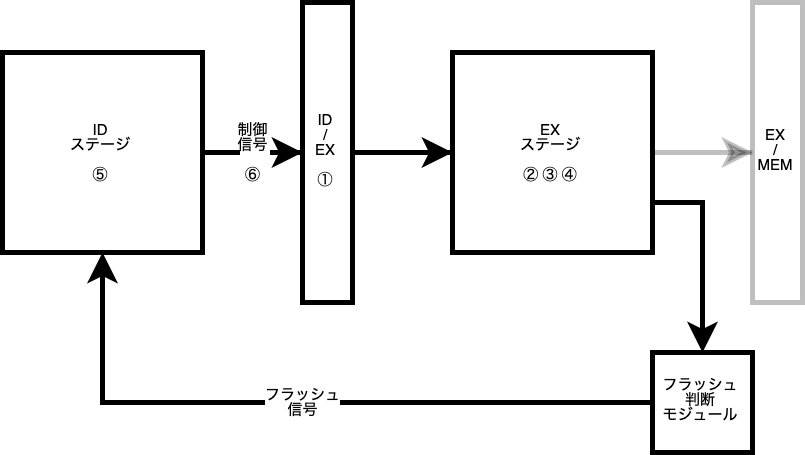
\includegraphics{../../images/flush_and_critical_path_before.png}
      }
      \caption{改善前}
      \label{fig:flush-and-critical-path-before}
    \end{subfigure}
    \begin{subfigure}{\columnwidth}
      \centering
      \resizebox{0.9\columnwidth}{!}{
        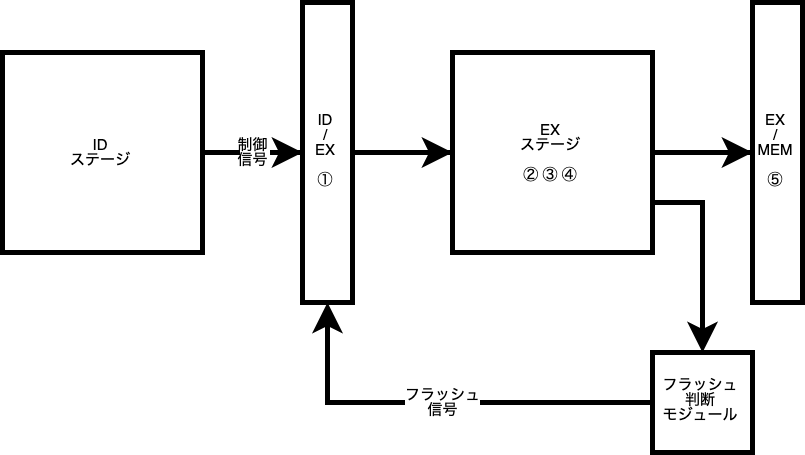
\includegraphics{../../images/flush_and_critical_path_after.png}
      }
      \caption{改善後}
      \label{fig:flush-and-critical-path-after}
    \end{subfigure}
    \caption{パイプラインフラッシュ処理の回路とクリティカルパス}
  \end{figure*}

  これを改善するために, パイプラインのフラッシュをステージ内ではなく, 
  パイプラインレジスタで行うようにした (図 \ref{fig:flush-and-critical-path-after}).
  改善後の回路では, たとえば ID ステージで「データメモリに対して書き込む」信号が生成されても, 
  EX ステージの分岐結果が「分岐する」なら, 
  その信号が ID/EX パイプラインレジスタに保存される前に, 「データメモリに対して書き込まない」へと無効化される.

  この改善によってプロセッサの最小動作クロック周期を $8\unit{ns}$ から $5\unit{ns}$ まで減らすことができた.
  改善によって得られたクロック周期は分岐予測導入前の $6\unit{ns}$ よりも短くなったため, 
  分岐予測機能を今回のプロセッサに導入することにした.

  \subsubsection{クリティカルパスの短縮後の論理合成}
  クリティカルパスの短縮を行った後の性能評価の結果を表 \ref{table:logic-synthesis-improved} に示す.
  クリティカルパスの短縮により, 分岐予測の実装によって $9\unit{ns}$ までに増えたクロック周期を
  $5\unit{ns}$ へと減少させることができた.

  \begin{table*}[t]
    \centering
    \caption{性能改善前後の論理合成の結果}
    \label{table:logic-synthesis-improved}
    \begin{tabular}{|c|r|r|r|}
    \hline
    プロセッサ & \multicolumn{1}{c|}{最小動作クロック周期 {[}\unit{ns}{]}} & \multicolumn{1}{c|}{面積 {[}$\unit{\um}^2${]}} & \multicolumn{1}{c|}{消費電力 {[}\unit{\mW}{]}} \\ \hline
    分岐予測実装前 & 6 & 357534.7228 & 7.5732 \\
    分岐予測実装後 & 9 & 936675.8334 & 10.6318 \\
    クリティカルパス短縮後 & 5 & 764805.1213 & 15.3567 \\ \hline
    \end{tabular}
  \end{table*}

\end{document}
